% Standalone source of the contracted-sector diagrams of the bubble time kernel
% (Sec. 5): the Top sector keeps the circular loop; pinching one propagator
% merges the two vertices and leaves the other propagator as a circular tadpole
% on the single merged component.
% Compile: pdflatex fig_bubble_sectors.tex   (included by paper.tex)
\documentclass[tikz,border=6pt]{standalone}
\usetikzlibrary{calc,positioning}
\begin{document}
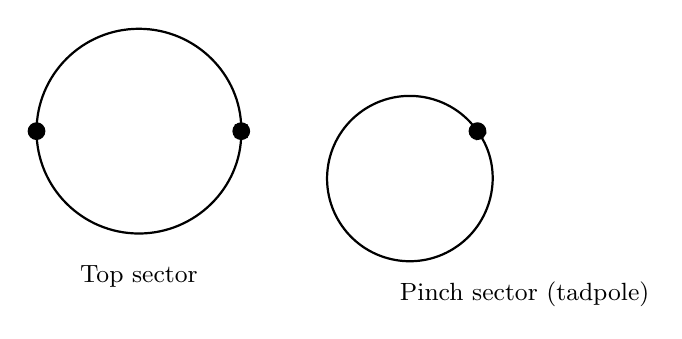
\begin{tikzpicture}[
  every node/.style={inner sep=1.5pt},
  dot/.style={circle,fill=black,draw=black,minimum size=6pt,inner sep=0pt},
  lab/.style={font=\small,anchor=north},
]
  % ============ Top sector ============
  \begin{scope}[shift={(0,0)}]
    \node[dot] (v1) at (0,0) {};
    \node[dot] (v2) at (2.6,0) {};
    \draw[->,thick] (v1) arc[start angle=180,end angle=0,radius=1.3];
    \draw[->,thick] (v1) arc[start angle=180,end angle=360,radius=1.3];
    \node[lab] at (1.3,-1.65) {Top sector};
  \end{scope}
  % ============ Pinch sector (tadpole) ============
  \begin{scope}[shift={(5.6,0)}]
    \node[dot] (t) at (0,0) {};
    \draw[->,thick] (t) arc[start angle=35,end angle=395,radius=1.05];
    \node[lab] at (0.6,-1.85) {Pinch sector (tadpole)};
  \end{scope}
\end{tikzpicture}
\end{document}
